%%%%%%%%%%%%%%%%%%%%%%%%%%%%%%%%%%%%%%%%%
% Thin Sectioned Essay
% LaTeX Template
% Version 1.0 (3/8/13)
%
% This template has been downloaded from:
% http://www.LaTeXTemplates.com
%
% Original Author:
% Nicolas Diaz (nsdiaz@uc.cl) with extensive modifications by:
% Vel (vel@latextemplates.com)
%
% License:
% CC BY-NC-SA 3.0 (http://creativecommons.org/licenses/by-nc-sa/3.0/)
%
%%%%%%%%%%%%%%%%%%%%%%%%%%%%%%%%%%%%%%%%%

%----------------------------------------------------------------------------------------
%	PACKAGES AND OTHER DOCUMENT CONFIGURATIONS
%----------------------------------------------------------------------------------------

\documentclass[a4paper, 11pt]{article} % Font size (can be 10pt, 11pt or 12pt) and paper size (remove a4paper for US letter paper)

\usepackage[protrusion=true,expansion=true]{microtype} % Better typography
\usepackage{graphicx} % Required for including pictures
\usepackage{wrapfig} % Allows in-line images
\usepackage{color}
\usepackage{gensymb}
\usepackage{mathpazo} % Use the Palatino font
\usepackage[T1]{fontenc} % Required for accented characters
\linespread{1.05} % Change line spacing here, Palatino benefits from a slight increase by default

\makeatletter
\renewcommand\@biblabel[1]{\textbf{#1.}} % Change the square brackets for each bibliography item from '[1]' to '1.'
\renewcommand{\@listI}{\itemsep=0pt} % Reduce the space between items in the itemize and enumerate environments and the bibliography

\renewcommand{\maketitle}{ % Customize the title - do not edit title and author name here, see the TITLE block below
\begin{flushright} % Right align
{\LARGE\@title} % Increase the font size of the title

\vspace{50pt} % Some vertical space between the title and author name

{\large\@author} % Author name
\\\@date % Date

\vspace{40pt} % Some vertical space between the author block and abstract
\end{flushright}
}

%----------------------------------------------------------------------------------------
%	TITLE
%----------------------------------------------------------------------------------------

\title{\textbf{Research Internship 1st Report}\\ % Title
Reinforcement Learning Overview \\and Tactile Reward Setting} % Subtitle

\author{\textsc{Tianming Qiu} % Author
\\{\textit{Institute for Cognitive Systems}}} % Institution

\date{\today} % Date

%----------------------------------------------------------------------------------------

\begin{document}


\maketitle % Print the title section


\section{Reinforcement Learning Overview} 
Some basic knowledges following are from Sutton's \textit{Reinforcement learning: An introduction}\cite {sutton1998reinforcement} and UCL course on RL given by David Silver. 

\subsection{Markov Decision Process}
A Markov decision process is a discrete-time state transition system. It can be described formally with 5 components as a 5-tuple $(\mathcal{S,A,P}, r,\gamma)$. 

$\mathcal{S}$ represents state space, 
$\mathcal{A}$ is action space, 
$\mathcal{P}$ means transition probability. 
If the transition probability satisfies $P(s_{t+1}|s_{t})=P(s_{t+1}|s_{t},s_{t-1},\dots,s_{1})$, that means it satisfies Markov property. Then this decision process is called Markov decision process. $r$ is reward.
$\gamma$ is a discount factor.

\subsection{Model-based Dynamic Programming}
'Model-based' means the knowledge of environment is known, mathematically means the transition probability matrix $\mathcal{P}$ and reward $r$ are already known. 
Two widely-used algorithms regarding dynamic programming are:
\begin{itemize}
\item Value iteration
\item Policy iteration
\end{itemize}
\subsection{Model-free Reinforcement learning: MC and TD}
\subsubsection{Monte-Carlo Reinforcement Learning}
Monte-Carlo method has no knowledge of MDP transitions and rewards. It learns directly from episodes of experience and the episodes are all complete, that is different from TD learning methods. The idea of Monte-Carlo method is $value = mean_return$, which is in the algorithm represented as:
\vspace{3mm}

Update value $V(S_{t})$ toward \textit{actual} return \textcolor{red}{$G_{t}$}:

\quad \quad $V(S_{t}) \leftarrow V(S_{t}) + \alpha (\textcolor{red}{G_{t}} - V(S_{t}))$ 

\subsubsection{Temporal-Difference Learning}
Same as MC, TD learning also has no knowledge of MDP transitions and rewards, it has to estimate value function from episodes of experience as well. The different is TD learns from \textit{incomplete} episodes. 
\vspace{3mm}

Update value $V(S_{t})$ toward \textit{estimated} return \textcolor{red}{$R_{t+1}+\gamma V(S_{t+1})$}:

\quad \quad $V(S_{t}) \leftarrow V(S_{t}) + \alpha (\textcolor{red}{R_{t+1}+\gamma V(S_{t+1})} - V(S_{t}))$ 

\vspace{3mm}
Above shows the similarity and difference between MC and TD learning. Also there are two main TD learning methods: 
\begin{itemize}
\item ON-policy: Sarsa
\item OFF-policy: Q-learning
\end{itemize}



\subsection{Q-learning}
Q-learning is most widely-used reinforcement learning algorithm, which is a kind of TD-learning.
Following is the algorithm:
\begin{center}\textbf{Q-learning: An off-policy TD control algorithm}

\vspace{1.5mm}

\fbox{\parbox{\textwidth}{Initialize $Q(s,a)$, $\forall s \in \mathcal{S}$, $\forall a \in \mathcal{A}$, arbitrarily, and $Q($terminal-state,$\cdot)=0$

Repeat (for each episode):

\quad\quad Initialize $S$

\quad\quad Repeat (for each step of episode):

\quad\quad \quad\quad Choose $A$ from $S$ using policy derived from $Q$ (e.g., $\epsilon$-greedy)

\quad\quad \quad\quad Take action $A$, observe $R$, $S'$

\quad\quad \quad\quad $Q(S_t,A_t)\leftarrow Q(S_t,A_t)+ \alpha [ R_{t+1} + \gamma \max \limits_{a}Q(S_{t+1},a)-Q(S_t,A_t)]$

\quad\quad \quad\quad $S\leftarrow S'$

\quad\quad Until $S$ is terminal
}}

\end{center}
\subsection{Deep Q Network}
If the state space is very big even against infinite, it will be trouble to use traditional q-learning method. Minh introduced a combination of deep learning network with q-learning called DQN algorithm.\cite{mnih2015human}
And this method works pretty well in Atari and Alpha Go. It stores transition $(s_{t},a_{t},r_{t+1},s_{t+1})$ in replay memory $\mathcal{D}$, and uses neuronal network to calculate Q values.
%------------------------------------------------

\section{Tactile Reward and Modeling} 

\subsection{Task}
\begin{figure} % Inline image example
  \begin{center}
    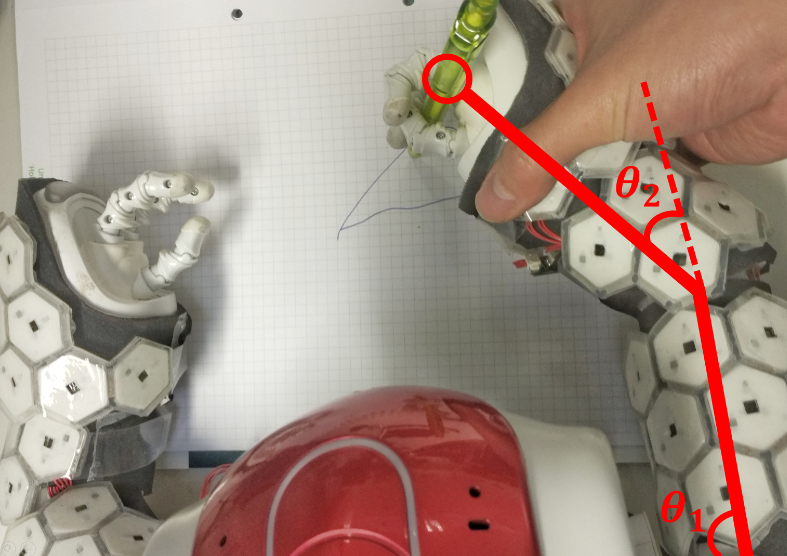
\includegraphics[width=0.6\textwidth]{task.png}
  \end{center}
  \caption{Draw a Triangle}
  \label{fig:task} 
\end{figure}

A very first the task could be train the NAO to draw a triangle like in figure \ref{fig:task}. Human will catch the robot hand and give the tactile feedback when robot is drawing. At the very beginning, the freedom of robot arm will be dropped to 2. Only shoulder and elbow joints will be used and two variables $\theta_1$ and $\theta_2$ can be changed and will be learned.

Further the task could be write letters following a personal font. And like images style transfer \cite{johnson2016perceptual} we could do something 'fonts' transfer for robot manipulation. This part I am not familiar with, just a simple idea.

\subsection{MDP Modeling}
\begin{itemize}
\item \textbf{States}: The ranges of both $\theta_1$ and $\theta_2$ are nearly 90\degree and they will be discretized into 90 levels. The state space will be $90 \times 90 = 810$ dimensions. It is already very large, maybe some methods should be taken to reduce the dimension. Or directly use DQN. 

\item \textbf{Actions}: $\theta_{i} = \theta_{i} \pm 1 \degree$ 
\item \textbf{Transition probability}: Joint angles will be read from NAO itself and $\mathcal{P}$ will be unknown before. This is a model-free problem.
\item \textbf{Reward}: Tactile reward can be written as a average force value feedback:
\[
r=-\frac{1}{N}(\sum_{i=1}^{N} f_{i}-f_{0})^2 
\]
wihch $f_{i}$ means the force data form the ith skin cell and $f_{0}$ means the average force when human just catches the NAO's hand and no guidance or pressure would like to give.
$N$ is the total number of skin cells.
\begin{figure} % Inline image example
  \begin{center}
    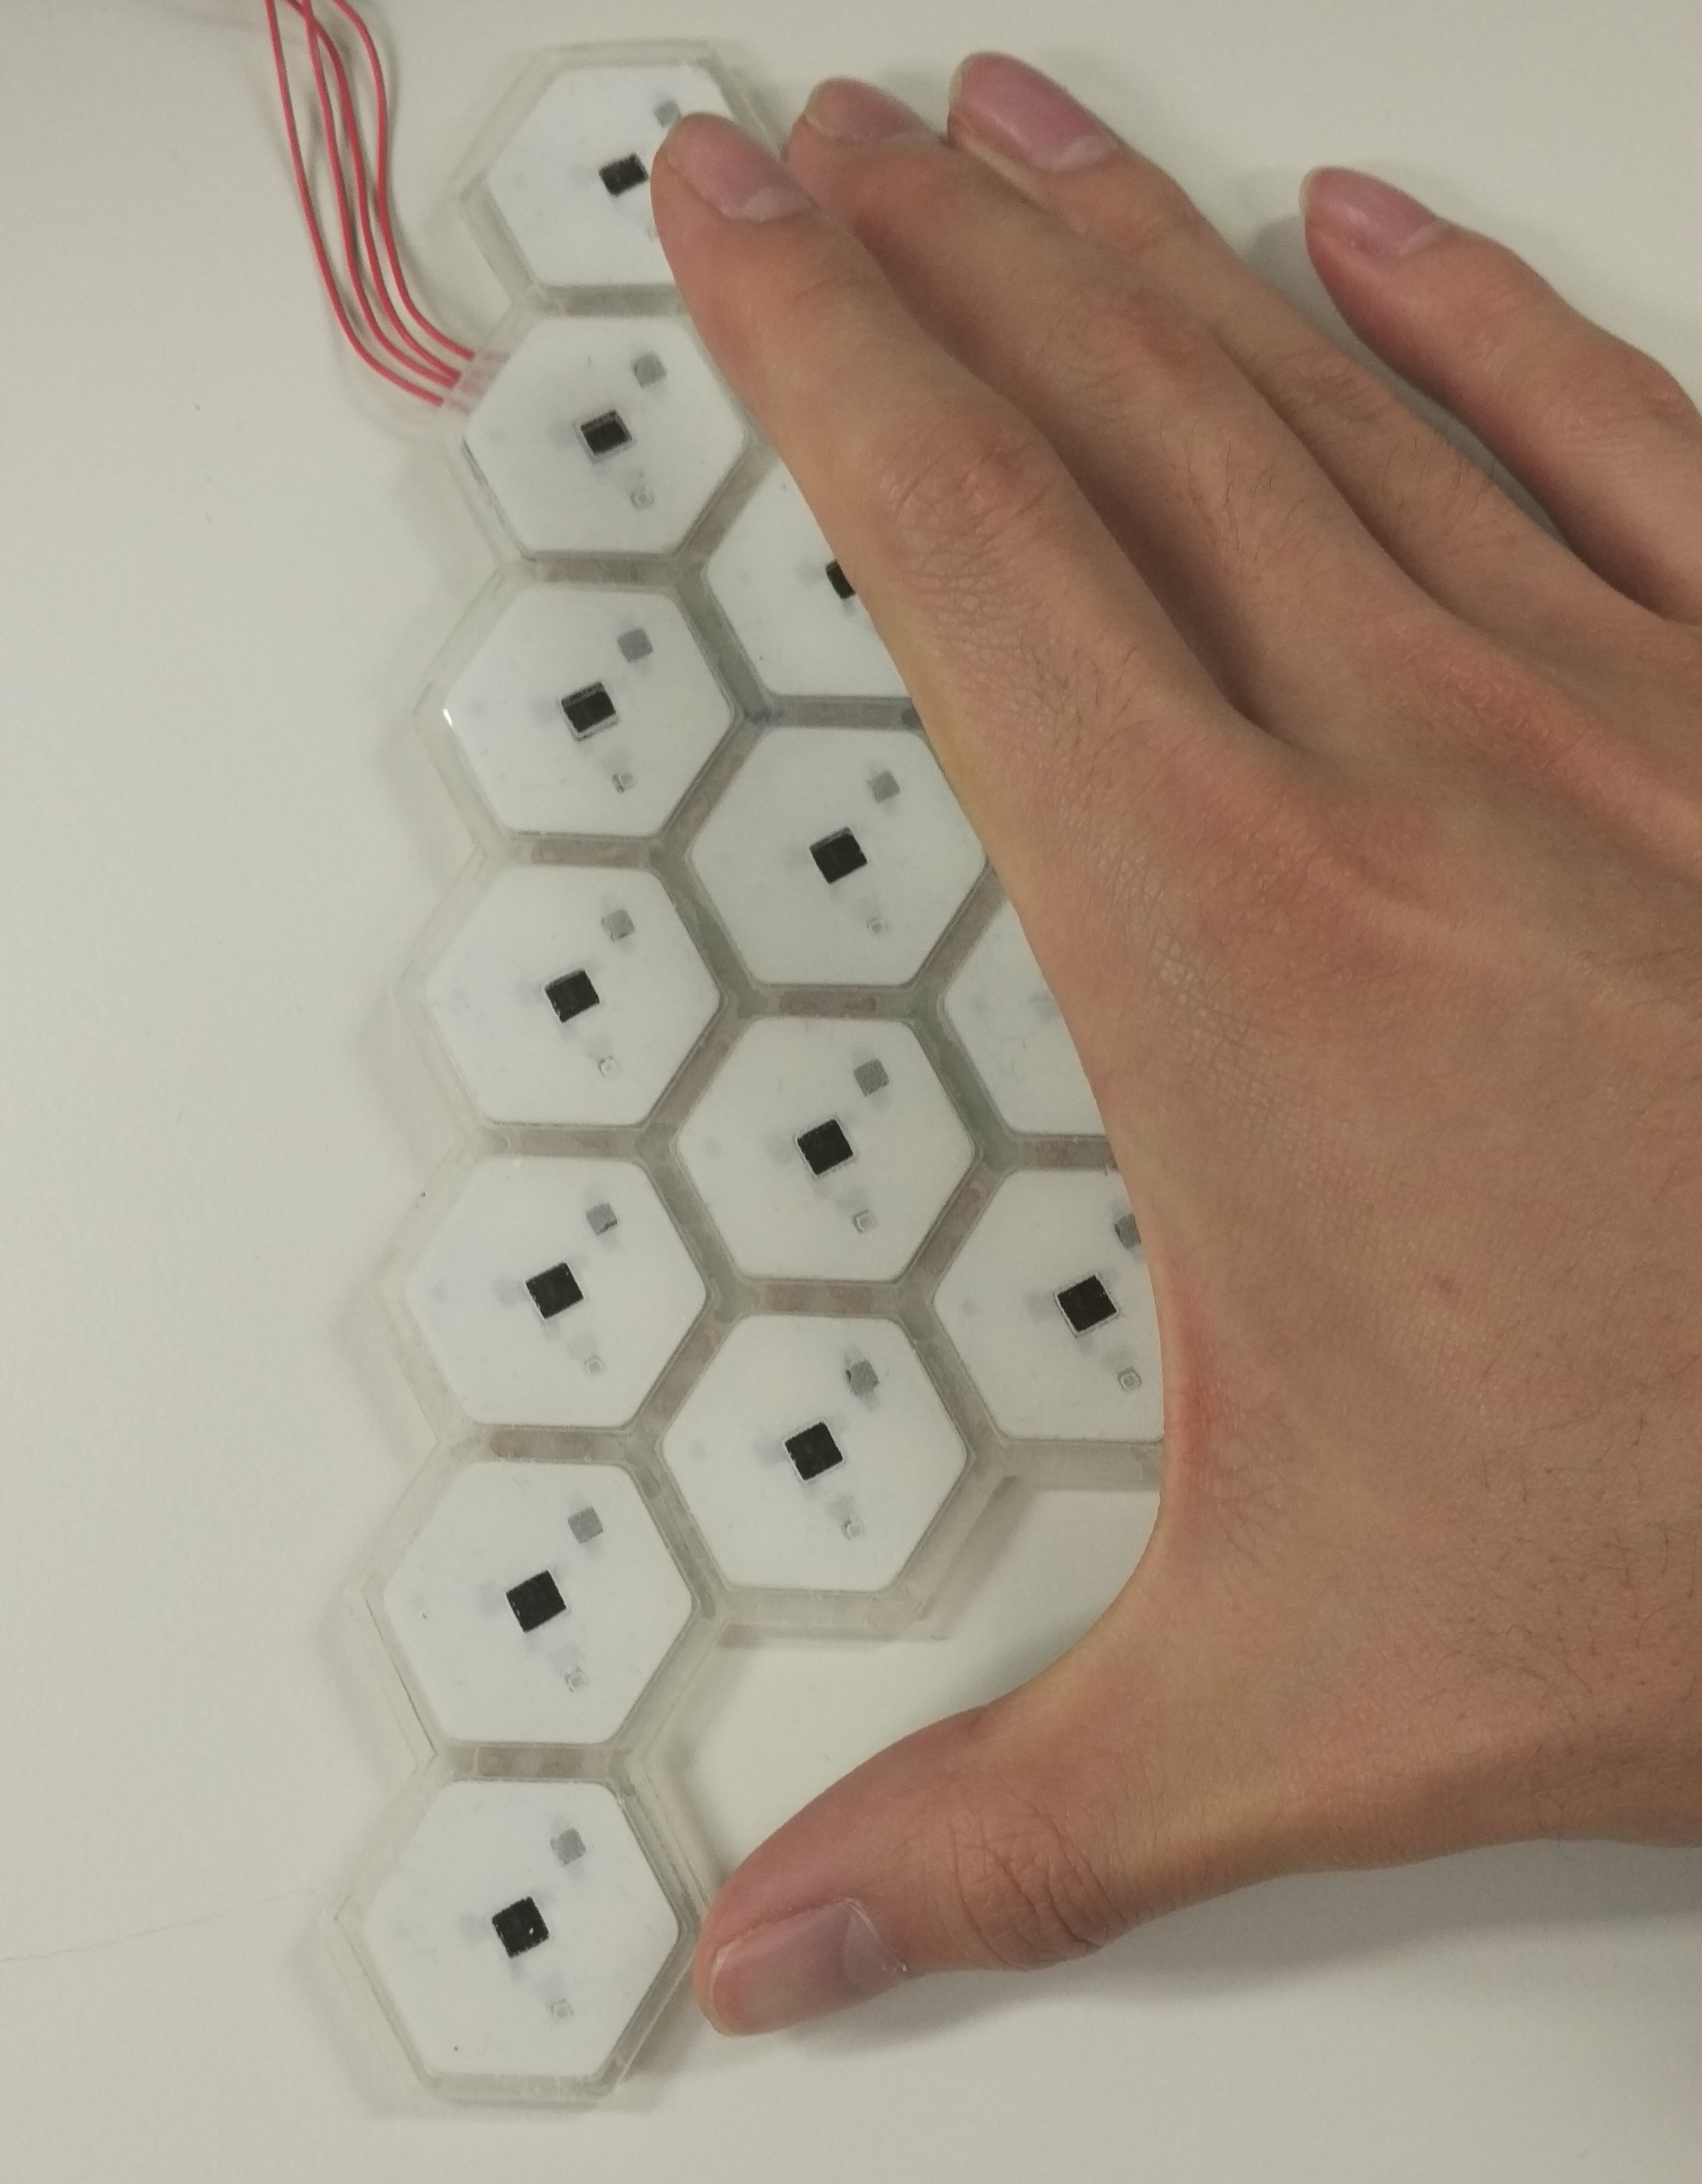
\includegraphics[width=0.4\textwidth]{skin.jpeg}
  \end{center}
  \caption{Artificial Skin Cell}
  \label{fig:skin} 
\end{figure}

In figure \ref{fig:skin} the skin around one hand include 14 skin cells and fit the size of human beings' hand. So it could record the each accurate change of human hand. 
\item \textbf{Discount factor}:  $\gamma$ will be temporarily chosen as 0.9.
\end{itemize}


\section{Future Plan }

\subsection{Manipulate Q-learning} 
I am not familiar with DQN, so I would like to manipulate the traditional Q-learning on NAO at first.

\subsection{Modify the MDP Model}
Reward function will influence the result a lot. I am not sure weather the modeling is suitable or not. And I also have 3-4 different ideas about how to represent the state space. So I need to first run some codes and find the issues, then make some necessary changes. 

\subsection{DQN}
Since robot arm has a continuous state space or the discretized state space are super large, DQN method need to be considered and it is proved by Alpha Go and Google's robot arm picking up manipulations\cite{gu2017deep}. 

\subsection{Add a Guidance like PbD?}
For reinforcement learning, if the robot arm fails to draw a pre-defined shape it will end an episode. I am figuring out can I give some guidance through tactile sensors and how, something like \textit{Programming by Demostration}\cite{billard2008robot}.

\subsection{More Functions of Artificial Skin}
Consider about more manipulations on artificial skin and some further task. For example, instead  of average force value how to give the direction feedback through different skin cell?


%----------------------------------------------------------------------------------------
%	BIBLIOGRAPHY
%----------------------------------------------------------------------------------------

\bibliographystyle{unsrt}

\bibliography{sample}

%----------------------------------------------------------------------------------------

\end{document}